

\textcolor{red}{Bring it back to the intro - our job is to document evolutionary history, and we need sound scientific methods for doing so.  OHara chronicle vs. history is empirical model vs. causal hypothesis.  Then introduce the sections - first, major conclusions and highlighting unique contributions, then future research, and then final thoughts.}


\section{Conclusions and Contributions}\label{conc:sec:research-conclusions}

\subsection{Microevolutionary Cultural Transmission Models in Archaeology}\label{conc:sec:conc-microevolutionary}

Despite the fact that archaeology understands itself as studying cultural \emph{change} through the archaeological record, we routinely (and often inadvertently) find ourselves describing the past in ways that are synchronic and essentialized.  Even though Nels Nelson \citeyearpar{Nelson1916} clearly articulated a diachronic and continuous understanding of change in artifact styles in his work at San Crist\'obal, later pratice in ``culture history'' framed our knowledge of the past as a series of synchronic snapshots.  \emph{Change} through time became represented as mere \emph{difference} between period or phases, and theoretical effort shifted to the reconstruction of the ``Indian behind the artifact'' \citep[79]{braidwood1959archeology}.  

The pull of synchronic description and the reconstructionist enterprise of describing the state of a population at a moment in time is no accident---it is built into the way we perceive the world and organize our knowledge.   \citet{Dunnell1982} described the cognitive biases that lead to this tendency as our ``common sense'', which constructs views of the world consistent with the short time scales over which we need to perceive the world and adapt.  Social and cognitive psychologists have since begun to document the proximate causation for essentialized cognition in early development \citeeg{Rhodes13526,rhodes2017development,gelman2004psychological}.  

Indeed, our tendency to think about the world in synchronic and essentialized terms is so strong that Mayr, Lewontin, and others have argued that the primary revolution Darwin kicked off was not about evolution itself, or even the theory of natural selection, but by introducing ``population thinking'' as an alternative to the typological, essentialist thinking about species and the nature world that characterized pre-Darwinian biology \citep{Dunnell1982,lewontin1974darwin,Mayr1959typological}.  The ``materialist revolution,'' as Lewontin termed it, treated \emph{variation} as causal, rather than noise, and required one to think about change in fully diachronic terms.  Evolutionary archaeology began with Dunnell's articulation of exactly this point \citep{Dunnell1978,Dunnell1980,Dunnell1982,Dunnell1989} and yet, the application of cultural transmission models within evolutionary archaeological very quickly took on a synchronic, ``reconstructionist'' flavor.  

By adopting equilibrium models from classical population genetics, whether the Wright-Fisher model of drift or the social psychological models from Boyd and Richerson's justifiably influential work \citeyearpar{BR1985}, the very structure of the models themselves gave predictions for the stationary, unchanging state of a population.  Fitting such models to observational data requires treating our data ``as if'' they were a synchronic sample of a population at a moment in time, so that the observed frequency distribution can be compared to the theoretical one.  Nearly all of the microevolutionary program for cultural  transmission modeling in archaeology has proceeded in this way, until very recently.  

Chapter \ref{chap:intro} describes in more detail how, as researchers began to see conflicting results when reanalyzing the same canonical data sets over and over in their methodological papers, it became apparent that efforts to fit cultural transmission models to data led to ambiguous conclusions.  This realization led to serious discussion about equifinality between transmission models, and the causes of that equifinality \citep{barrett2019equifinality,kandler2019analysing,premo2010equifinality}.  The first set of questions that comprise this dissertation address this question:  how severe are  the equifinality problems faced by the microevolutionary approach?  Is it possible to distinguish between transmission models using coarse-grained data on frequencies of cultural traits in a population?  Archaeological data are ``coarse grained'' in two ways, both relevant to the microevolutionary program. 

The first is that archaeological observations are always diachronic in nature and inherently represent counts and frequencies that refer to depositional events over a duration.  Sometimes the duration might be short, as in the archaeological record of recent historical periods, or our samples of the record may represent millennia in a single assemblage. Second, frequencies of artifact classes or types represents samples of cultural behavior across some past population.  It is difficult to say how or whether we can measure internal variation within a population, except perhaps under very specific depositional conditions and perhaps historical contexts.  This means we typically lack information about individual variability below the level of the population, which has been highly successful in laboratory and living observational studies in identifying different modes of social learning.  Chapters \ref{chap:timeaveraging-paper} and \ref{chap:ctmixtures-paper} addressed each of these types of ``coarse graining'' on our ability to fit cultural transmission models.  I summarize their conclusions in turn.

\subsubsection{The Centrality of Time Averaging To Evolutionary Modeling}\label{conc:sec:conc-timeaveraging}

Chapter \ref{chap:timeaveraging-paper} examined the effect of time averaged observations on the observable statistics we use to measure goodness of fit between archaeological frequency distributions, and the theoretical models we employ as hypotheses.  Since most of our hypothesis tests or goodness of fit testing is related to the shape of frequency distributions, it is useful to understand first the effects of aggregation on diversity measures.  I found that richness is inflated in samples with longer duration compared to synchronic observations.  This has been obvious to archaeologists for a century, and is a principle reason why culture historians noted that assemblages used in seriation should be of equal duration.  But this fact takes on critical importance with most of our cultural transmission models, since the number of expected traits (or alleles, given their origin in population genetics) is the ``sufficient statistic'' at a given population size and mutation rate.  The ``evenness'' of frequencies is flattened with greater assemblage duration; this causes problems with neutrality tests that seek to employ the shape of the frequency distribution, including Ewens and Watterson's tests and Slatkin's ``exact'' tests for neutrality.  As a result, such tests display increased Type I error rates.  These conclusions, and the difficulties that time averaging presents for fitting microevolutionary models to data, have since been echoed by \citet{Premo2014} and \citet{perreault2018time}.  

Perhaps the most important contribution of Chapter \ref{chap:timeaveraging-paper} is the linkage between how long cultural traits persist in the record, and the timescale over which time averaging effects appear.  Assemblages whose duration is longer than the mean lifetime of the classes which analytically represent cultural variation will display increased richness, flattened diversity, and increased Type I error in ``neutrality tests.''  Assemblages whose duration is equal to the mean trait lifetime, or shorter, are not affected by time averaging in these ways measured here.  

This is an important result because archaeologists can, at the time of data collection and subsequent artifact analysis, exert some control over the effects that time averaging might have on our analyses.  Sometimes it is possible to control the degree to which we aggregate artifacts into ``assemblages'' for analysis both during fieldwork, and afterwards in an analytical manner.  Assemblage duration is not fully controllable in this manner, of course, but to date this has not be a variable which has entered into the application of cultural transmission analysis.  The combined results of my work on time averaging, along with results by \citet{Premo2014}, \citet{Porvcic2014}, and \citep{perreault2018time,perreault2019quality} suggest that it should be.

In like manner, we have partial control over the relative lifetimes of the artifact classes we use to measure cultural variation.  We must always remember that the classes and types whose frequencies we are comparing to transmission models are analytical constructions, rather than being inherent in the rocks and sherds we handle themselves \citep{Dunnell1971}.  Because we form the classes we then use for counting abundance and forming frequency distributions, we can vary classification ``level'' (\emph{sensu} \citealt{Dunnell1971}) and vary the amount of time over which we observe a class.  Varying the number of dimensions of variation in our classification will affect the measured ``lifetime'' of the classes themselves.  Individual attributes (or modes) belonging to a single dimension of variation (e.g., straight rims on ceramic bowls) may persist in the archaeological record for long periods of time (and, indeed, by themselves may occur in unrelated contexts, thus being non-homologous).  But when we combine dimensions of variation, say by constructing a ceramic classification by intersecting rim form with surface treatment with rim decoration, each combination of these dimensions tends to have a more restricted spatio-temporal distribution.  Since we can affect our classifications and the level of detail they differentiate, we have some ability to tune our observations of cultural trait frequencies in response to the level of temporal aggregation present in the archaeological deposits we seek to study.  

To date, research in the microevolutionary approach has focused on the models themselves, and not on how we form the empirical frequencies that models have been compared with.  Virtually all of the studies summarized in Chapter \ref{chap:intro} employ already published data, and do not attempt to reclassify or alter the way variants are tabulated.  In my own work, I began work on a simulation framework for tracking cultural variation at multiple classificatory levels during simulated evolution, available as open source software \footnote{See the Github repository \url{https://github.com/mmadsen/CTPy}, in the \emph{coarsegraining} module.}.   I return to the importance of classification level in Section \ref{conc:sec:future-design-space}, since we have not done enough to understand the effects of classification on how we can measure the history of cultural variation (the major exception being \citealt{Lipo2001}). 

The ability to control the coarse or fine grained level of our classifications may provide, in some empirical circumstances, the ability to examine microevolutionary questions, especially if combined by attention to temporal control during data recovery and careful design of an overall strategy for chronological control.  The relationship between duration and mean trait lifetime described here provide the tools to understand when the time averaging effects of aggregated, coarse grained observations will make it impossible to distinguish between hypotheses securely.  In Perreault's \citeyearpar{perreault2019quality} terminology, with sufficient temporal control and classificatory detail, microevolutionary hypotheses about cultural transmission may not be underdetermined in all cases.  But time averaging presents a significant and ever-present issue for model fitting in archaeology, whether for evolutionary modeling or faunal analysis.  The ubiquity of time averaging effects should be telling us something about the scales over which we can ask meaningful questions, as I discuss below.

\subsubsection{Coarse Grained Data Cannot Inform on Population Structure}\label{conc:sec:conc-ctmixtures}

Chapter \ref{chap:ctmixtures-paper} examined the second problem that the microevolutionary approach faces given only coarse grained data sources.  Since real human (and animal) populations are a mixture of individuals with different social learning strategies, we need to stop fitting models of single pure cultural transmission processes, and understand whether we can study \emph{variability} in social learning, since that variability is the raw material for future evolution of social learning capabilities themselves.  Thus, I examined whether it was possible to distinguish \emph{different} mixtures of social learning strategies with only population-level summary data, in the form of relative frequencies of artifact classes.

The results were not encouraging, if population level data are also subject to sample size effects and any temporal aggregation.  It proved possible in some cases to distinguish between mixtures of strategies and a population of the same size practicing unbiased copying, when the frequencies used were a complete census of the population, and when no aggregation was present.  With partial samples of the population, equifinality between models (even under the ideal circumstances of a simulation experiment) increased.  Similarly, when time averaging of observations is a factor, equifinality between model comparisons was strong, and with both factors, we are simply unable to distinguish between theoretical models with population-level data on trait frequencies.  This does not bode well for identification of microevolutionary models of transmission in most archaeological situations.  

This research makes several contributions.  First, it contributes to a growing literature on the need for ``thicker'' or more realistic cultural transmission models.  Leaving asides modeling at macroevolutionary scales for the moment, even within the microevolutionary approach we are seeing movement from simple synchronic models of psychological bias to diachronic, non-equilibrium models capable of incorporating history and change \citeeg{Kandler2013,kandler2018generative,kandler2019analysing,Rorabaugh2014}.  My work in Chapter \ref{chap:ctmixtures-paper} adds heterogeneity to this mixture of model elements.  \citet{Tostevin2012,tostevin2019content} adds explicit modeling of the \emph{content} of culturally transmitted knowledge, as does my work in Chapter \ref{chap:semanticaxelrod-paper} (see \ref{conc:sec:conc-structured}). 

\subsection{A Systematic Method for Measuring Equifinality and Underdetermination}\label{conc:sec:equifinality-underdetermination}

Second, the work in Chapter \ref{chap:ctmixtures-paper} describes an explicit method for detecting equifinality among theoretical models, as well as ways in which the spatiotemporal resolution, duration, or data collection treatments may affect where our data underdetermine those models.  I use the idea that models which are not equifinal will generate predictive data distributions (by whatever method, but typical via Monte Carlo sampling or simulation modeling) which can be distinguished by the \emph{Bayes classifier} for the model set.  The Bayes classifier is usually not possible to directly calculate or implement, but it can be well approximated by using machine learning classifiers with sufficiently high model capacity.  In this study, I examined classifier performance in distinguishing pairs of transmission models, with samples from the same predictive data but with differing sample sizes and amounts of temporal aggregation.  This combination of methods allows us to examine two questions simultaneously \begin{dissparalist}
\item are a set of models or hypotheses distinguishable \emph{even in theory}, given a set of observable variables
\item how do data collection treatments, or the empirical scale of our data in terms of resolution or duration, affect model identification
\end{dissparalist}?  This method is more general than cultural transmission modeling, and in fact should be a standard question we ask about theoretical models and our data at the outset of a research project.  As \citet{perreault2019quality} notes in his excellent recent book, far too much archaeological research is empirically insufficient because models are equifinal, or are underdetermined by any data we can feasibly collect.  

The work done by Kandler on diachronic, non-equilibrium models, as well as the work presented here on time averaging and equifinality of realistic social learning mixtures, point to the fact that the microevolutionary program, is not workable.  It is not a matter of ``correcting'' equifinalities with better statistical methods.  The strategy of attempting to fit synchronic, equilibrium models to coarse grained data of varying duration and temporal resolution is conceptually flawed.  We should leave it behind.

The strength of archaeology as an evolutionary discipline is time depth:  we study a record of how human behavior differs over space and has changed over time.  This requires us to construct models that are hypotheses about the evolutionary history of cultural variants in a region and over a period of time.  Our evolutionary models should be hypotheses about the trajectories that different models of cultural transmission and social learning take, over time scales which match the time scales at which we can realistically observe the process.  

\subsection{Seriation Graphs Are Evolutionary Chronicles at the ``Mesoscale''}\label{conc:sec:conc-seriation}

\citet{OHara1988}'s distinction between ``chronicle'' and ``history'' is a critical one.  Chronicles are ``the facts,'' while histories are explanations.  Histories provide causal narratives that purport to explain the chronicle of empirical observations. In Chapters \ref{chap:seriationcombinatorics-paper}, \ref{chap:multipleseriation-paper}, and \ref{chap:computational-metapopulation}, I explored how to \begin{dissparalist}
\item formalize a hypothesis about the regional history of community interaction and cultural transmission in the form of an ``interval temporal network'' model
\item construct seriation graphs which summarize the spatial and temporal history of how cultural traits varied 
\item develop statistical summaries of seriation graphs, for purposes of assessing goodness of fit between the empirical seriation and temporal network models
\end{dissparalist}.  In this structure, a set of interval temporal network models are the candidate ``histories'', and function as hypotheses.  Seriation graphs function as one kind of evolutionary chronicle; in this case, it is a chronicle about the spatial and temporal change that we see in the frequency of different cultural traits.  

In order for seriation graphs to function well as chronicles, they need to have rich enough state spaces that different causal histories will cause meaningful differences in the structure of the seriation solutions.  This is an important reason that Lipo and I moved to a graph representation from our former work building multiple independent seriations out of empirical datasets \citep{Lipo2015}.  But richness of structure means that seriations must incorporate many assemblages, not just a few.  Small seriation solutions will nearly always underdetermine any set of candidate hypotheses, because the models will often be equifinal across very small samples.  Thus, in Chapter \ref{chap:multipleseriation-paper}, I worked with Carl Lipo on developing more efficient criteria for seriating large sets of assemblages.  Our results with distance-minimization as the ordering criterion builds on earlier work by Kadane and Shepherdson, and in combination with our graph construction heuristics, yields the ability to easily analyze dozens of assemblages at a time and construction seriation graphs.  

Chapter \ref{chap:computational-metapopulation} represents an initial attempt to put the pieces described above together, and determine whether it is possible, in theory, to discern hypotheses about regional transmission history, using seriation graphs as the empirical unit of observation.  The results are positive and suggestive that further research would help outline the limits of the approach, and possibly improve discriminatory power between different classes of historical models.  I return to the next steps for this research program in Sections \ref{conc:sec:future-temporal-networks} and \ref{conc:sec:future-seriation-structure}.   

\subsection{Methods for Including Structured Information in Cultural Transmission Models}\label{conc:sec:conc-structured}

In addition to constructing better spatiotemporal models of cultural transmission at archaeological scales, we also need ``thicker'' descriptions (sensu \citealt{Geertz1973,gilbert1949concept}) of cultural variation and how social learning processes interact and coevolve with the \emph{content} of cultural variation.  Following ideas from \citet{mesoudi2008learning}, in Chapter \ref{chap:semanticaxelrod-paper} I considered how to build a model encapsulating the \emph{dependency structure} between traits in the form of a graph.  Transmission dynamics were then subject to that dependency structure as well as social learning rules.  Two types of social learning rule were then compared in a modified Axelrod model:  individual innovation, as compared to teacher-led imitation.  The theoretical results show that, as one might expect, formal instruction or tutoring results in deeper, more complete cultural repertoires, in comparison to pure imitation and individual trial-and-error learning.  This provides additional theoretical support for the idea that ``behavorial modernity,'' the explosion of complexity and variety seen in Upper Paleolithic hominids, may be the result of the coevolution of new forms of social learning with the increase in complexity of the content of cultural variants.  

At a methodological level, this work contributes new ways of modeling cultural transmission such that we can create credible hypotheses for how social learning rules and content can evolve together.  This is necessary if we are going to move beyond formal, very abstract models for cultural transmission, and actually explain the evolutionary history of blade tools, for example, or the evolution of different kinds of ceramic technologies.  The effort to construct thicker models has been championed by \citet{tostevin2019content} in archaeology, following the critically important work of William Wimsatt and colleagues \citep{wimsatt2007reproducing,wimsatt2019articulating}.  I discuss some possible future research directions in Section \ref{conc:sec:future-design-space}.

\section{Next Steps and Future Research}\label{conc:sec:future-research}

The major goal of my dissertation research is to examine whether we can improve the empirical sufficiency of cultural transmission research in archaeology by \begin{dissparalist}
\item understanding the sources of equifinality between models
\item modeling cultural transmission at spatial and temporal scales appropriate to the coarse grained nature of archaeological data
\item selecting empirical observable units (such as seriation graphs) which display enough variation between models, that our hypotheses are not underdetermined
\end{dissparalist}.  The conclusions just described show, I believe, some success in achieving all three goals.  Nevertheless, some of the approaches I employed, such as the use of temporal networks and seriation graphs in Chapter \ref{chap:computational-metapopulation} remain in their infancy, with many questions still to answer and refinements possible.  In this section, I describe next steps for several of the methods and approaches used in previous chapters. 

\subsection{Further Development of Temporal Network Models as Evolutionary Hypotheses}\label{conc:sec:future-temporal-networks}

In Chapter \ref{chap:computational-metapopulation}, I examined the idea that we could represent a diachronic hypothesis about the history of cultural transmission in a region in the form of a so-called ``temporal'' or ``time-varying'' network.  Temporal networks are general graphs, in the mathematical sense, with vertices and edges, but extended in time.  Each vertex and edge carries information about the times at which each existed.  Thus, over time, not only does the pattern of connectivity between vertices change, but the vertices themselves can arise, persist, and then go away.  Such models, because edges do not represent instantaneous contacts but longer durations, are called ``interval temporal networks.''  

I proposed that interval temporal networks (or ITNs) were a good tool for representing long term change in cultural transmission patterns between sedentary, nucleated communities.  The ITN functions as a formalization of a standard ``metapopulation'' modeling framework, in which discernible subpopulations can be identified and sampled, and have sufficient persistence that one could (in theory) measure migration rates between the subpopulations.  Not all of the empirical situations we wish to study as archaeologists fit into a metapopulation modeling strategy, however, and thus interval temporal networks will not be a good tool for representing evolutionary hypotheses in all situations.  Interval networks would not be a good structural model for transmission in highly mobile populations or dispersed hunter gatherer communities, for example.  Given how difficult it is to describe residential and community patterning in the deep Paleolithic record, we would need different empirical models for such situations, which perhaps look more like continuous fields with gradients rather than graphs with nodes and edges. 

Within the class of problems for which interval temporal networks are appropriate, there are several avenues to follow and improve upon the results reported here.  These include:

\begin{itemize}
    \item Understanding how to characterize equivalence classes of temporal network structures, in the same way that we can order or classify static graphs;
    \item Describe equivalence classes of network structures that have similar behavior under transmission or diffusion processes
\end{itemize}.

The first element involves understanding good ways to characterize meaningful differences in interval graphs.  In Chapter \ref{chap:computational-metapopulation} I did not directly analyze the temporal network models themselves, instead looking for the \emph{effect} their structure may have on transmission via seriations.  This approach, derived from my earlier work on ways to characterize equifinality (see Chapter \ref{chap:ctmixtures-paper}), is useful but highly indirect and computationally expensive.  We can complement the approach I took here with a direct study of the interval temporal networks that form our transmission scenarios.  

For static graphs, there are many results in graph theory that help characterize equivalence classes of graphs.  In particular, functions of the Laplacian spectrum define classes of structures, as do the eigenvalues of the adjacency matrix.  The ``energy'' of a graph (i.e., the sum of the eigenvalues of the adjacency matrix) appears to be strongly related to how the graph can be decomposed into subgraphs with differing structure (e.g., cycles, cliques, trees) \citep{estrada2017meaning,gutman2006laplacian}.  We also know, for example, We know that trees which have 4 or 5 distinct eigenvalues (at a given diameter) are completely characterized by their normalized Laplacian spectrum \citep{braga2015trees}.  That is, each distinct set of eigenvalues forms a distinct and distinguishable set of tree structures.  The ability to understand structural equivalence classes is important for understanding when we should see differences in the \emph{behavior} of a cultural transmission process across a set of network structures, since a large body of research has shown how graph topology affects diffusion-like processes on static graphs (see reviews in  \citealt{Castellano2006,Durrett2007,grimmett2018probability,szabo2007evolutionary}).

For time varying or temporal graphs, we are beginning to understand their structural properties \citep{nicosia2013graph,nicosia2012components}, especially given strong interest by computer scientists in using temporal contact networks to study consensus algorithms, distributed systems design, and mesh network design.  Similarly, given the importance of time varying contact networks in epidemiology, we are beginning to understand the behavior of diffusion processes across contact networks \citep{liu2013contagion,pare2017epidemic,liu2014social,uribe2019non,santoro2011time}.  Most of this work has focused on ``contact'' networks where edges represent short-duration events, so there is a need to examine the degree to which the behavior of diffusion processes on interval networks may differ from contact networks.  

Second, given a general understanding of how diffusion processes (including epidemics, cultural transmission, population genetics) operate on interval networks, we can return to the general approach taken in Chapter \ref{chap:computational-metapopulation} and examine more systematically which transmission scenarios we can distinguish.  To answer archaeological questions about ``complex societies,'' for example, we would like to be able to formulate transmission scenarios where ``hierarchy'' exists, and the transition from flatter ``nearest neighbor'' and ``small world'' patterns of connectivity to hierarchical patterns of interaction.  

\subsection{Statistical Properties of Seriation Graph Solutions and Transmission Scenarios}\label{conc:sec:future-seriation-structure}

In order to perform statistical analysis on seriation solutions, including using classifier models to under equifinality, or clustering algorithms to understand similarities in structure, we need to extract summary statistics from seriation graphs.  In Chapter \ref{chap:computational-metapopulation} I focused on the ``Laplacian spectrum'':  the set of eigenvalues and their multiplicities for the Laplacian matrix of a graph.  The Laplacian matrix for a general graph incorporates information about the pattern of edge connections through the adjacency matrix, and the density of connectivity (or ``branchiness'', for trees) through the degree matrix.  I employed the eigenvalues of the Laplacian as a set of independent or predictor variables that I used to train a classifier model, measuring the ability to cleanly separate different graph structures and ``predict'' the true data generating model underlying the seriation graph.  This was fairly successful but it is something of a ``black box'' approach, which is suitable for measuring the \emph{presence} of equifinality but without providing much guidance on why the outcomes of simulated transmission on different transmission scenarios might be distinguishable or not.  

One thing that the approach taken in Chapter \ref{chap:computational-metapopulation} did not clarify is the degree to which seriation graphs might not vary enough in their Laplacian spectra to distinguish between data generating processes.  How large is the ``state space'' formed by possible eigenvalue spectra for all trees on N vertices?  It may turn out that there is enough variation to differentiate transmission scenarios which are extremely different in their structure:  for example, nearly regular graphs of the ``nearest neighbor'' type, and a lineage splitting model which contains separate components.  But seriation graphs may have enough structural similarity across transmission scenarios that they underdetermine other comparisons:  nearest neighbor and small world graphs, versus hierarchical structures, as a possible example.  But these are exactly the kind of scenarios we wish to study at the mesoscale, in order to resolve questions about Mississippian ``complexity''.  

\begin{figure}[p!]
  \centering
  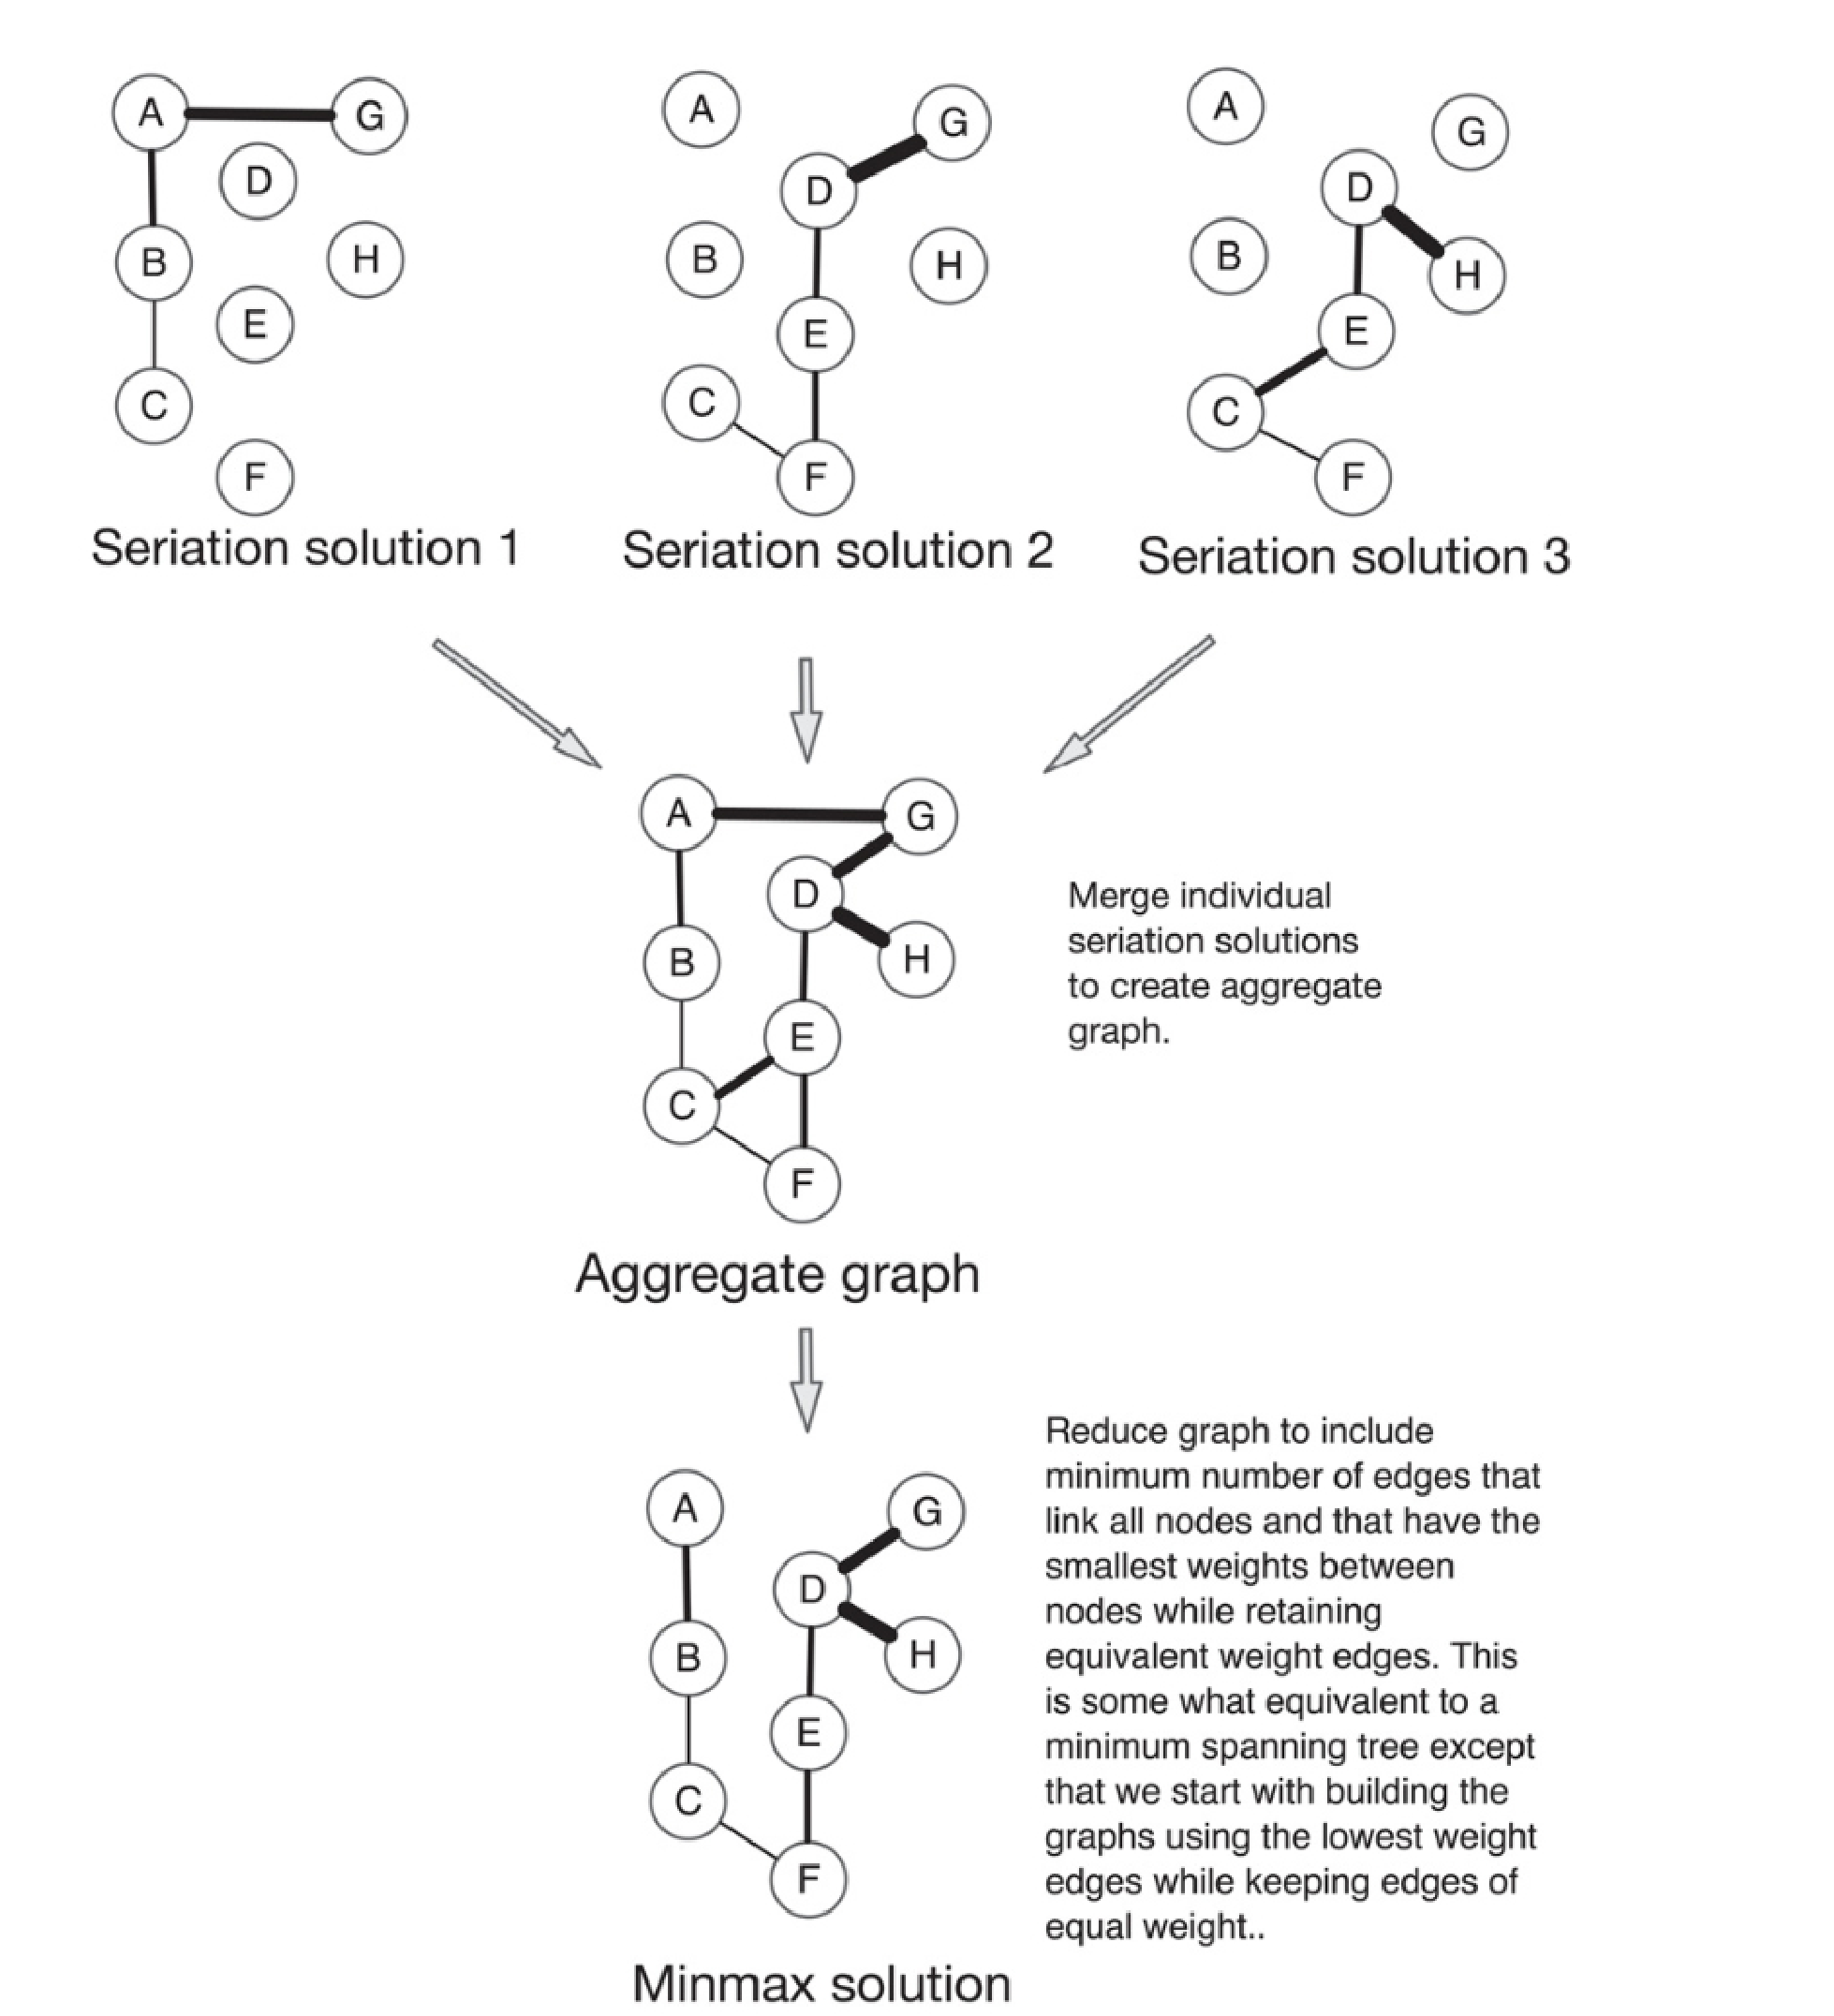
\includegraphics[scale=0.4]{graphics/conclusion/lipo2015-figure6-minmax.pdf}
  \caption{Seriation graph creation steps.  In this example, we begin with the graph representation of three valid seriation solution fragments (1-3) for a set of 9 assemblages (A-I).  In the figure, the thickness of the edges reflects the summed difference in frequencies between each pair of assemblages.  Each solution represents a valid and unique seriation.  To combine these three possible solutions into one overall solution, we first take the union of the partial graphs to create a single aggregate solution that is composed of all vertices and edges from the individual subsolutions.  Using the aggregated graph or ``sumgraph'', we then reduce to a final seriation solution by including the fewest edges that can be made between all vertices and starting with the edges with the smallest weight (the sum of frequency differences).  Edges are added sequentially ranked by total frequency difference until the vertices form a single connected three.  Edges with equivalent total weight are retained.  Reprinted from Figure 6, \citep{Lipo2015} under the terms of the Creative Commons Attribution License \url{https://creativecommons.org/licenses/by/4.0/}.}
  \label{conc:fig:minmax-seriation}
\end{figure}

It is possible to study other representations of seriation data as well which might contain more structure.  Our IDSS seriation algorithm \citep{Lipo2015} by default produces solutions which represent the ``minmax'' solution:  the largest set of assemblages that can form a valid solution, linked by edges which represent the smallest differences between class frequencies among adjacent vertices (Figure \ref{conc:fig:minmax-seriation}).  This ``minmax'' solution graph, whether constructed using unimodality as the ordering criterion or simple distance minimization (as described in Chapter \ref{chap:multipleseriation-paper}), represents a kind of minimal spanning tree which accounts for both spatial and temporal effects on ordering assemblage frequencies.  

That minimum spanning tree is constructed by \emph{pruning} edges from an intermediate representation which is the union of all valid subsolutions (Lipo and I dubbed this the ``sumgraph'' or ``aggregrate'' graph representation).  If the criterion being used is unimodality, the sumgraph will represent only those links where unimodal solutions could be found, and will be denser than a tree but sometimes sparser than the complete graph over N vertices.  The sumgraph records more similarity information than a ``minmax'' solution tree, and can have loops, cliques, and richer overall structure.  Because the graph structures are not strict trees, and can have richer connectivity patterns (which can vary in different areas of the solution), the Laplacian spectra should exhibit more variation.  This creates a large space of variation within which we might distinguish between hypotheses in assessing equifinality, and potentially clearer ability to fit empirical data to different models.  I have done some work repeating the experiments of Chapter \ref{chap:computational-metapopulation} with sumgraphs rather than minmax seriation trees, and the results seem promising.  

\subsection{Classification and Modeling Design Space}\label{conc:sec:future-design-space}

We always measure cultural variation, and map its spread through space and history through time, by examining the prevalence of archaeological classes of types \citep{Dunnell1971}.  These classes are always analytical constructions, even if in practice archaeologists frequently employ standard classifications in a given region whose origins are a mixture of analysis and common sense.  Since those classes are constructions, it is clear that ``Baytown Plain'' or ``Elko corner-notched'' are not really units of transmission, in the sense that the attributes denoted by those types were always learned or copied together.  And yet, in much of the published literature on cultural transmission modeling in archaeology, we end up treating types as if they were units of transmission.  This can obscure our ability to differentiate hypotheses about evolutionary history.  



\begin{figure}[ht!]
  \centering
  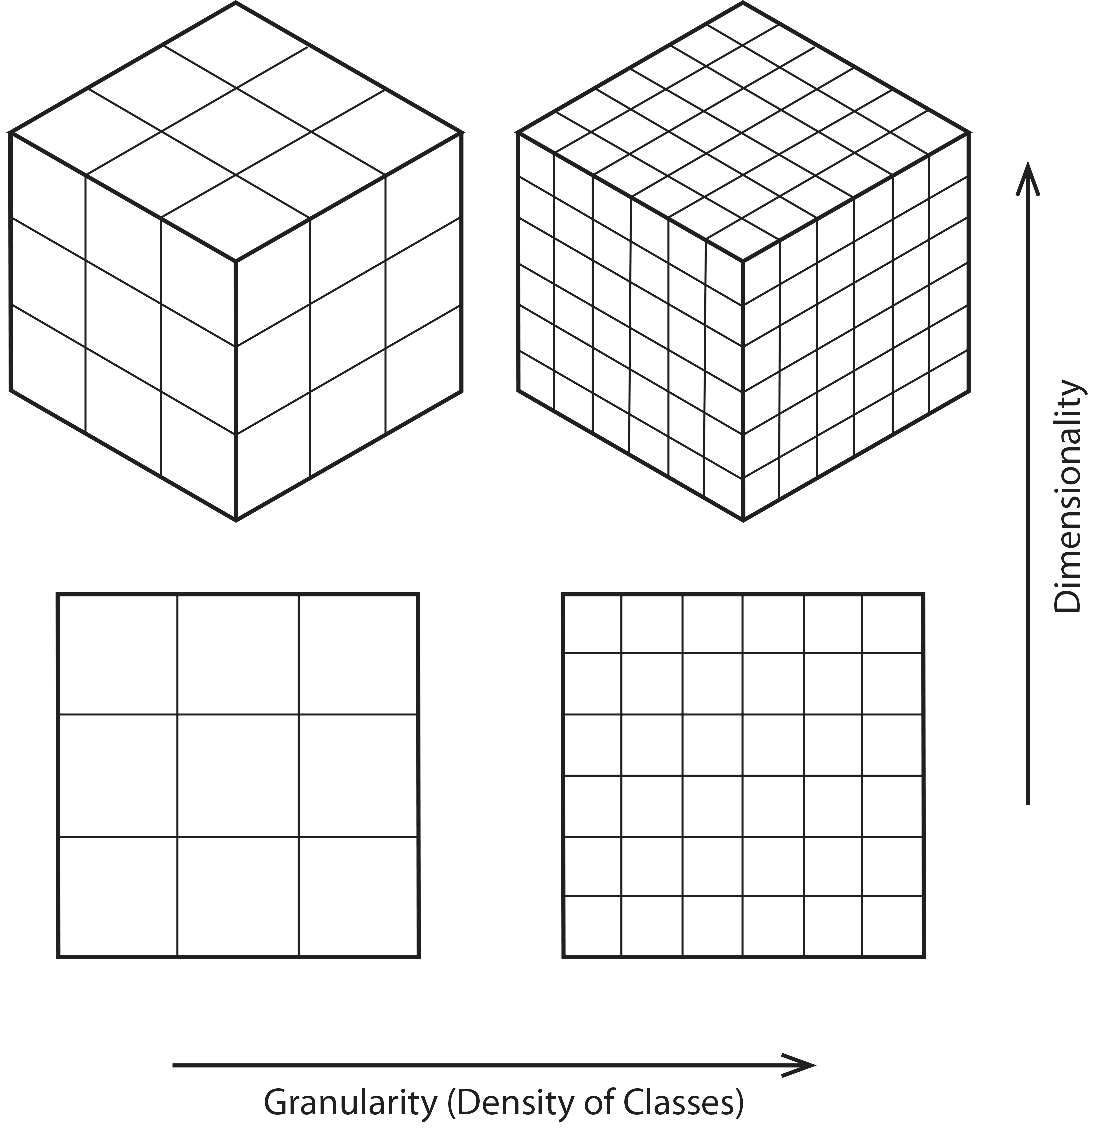
\includegraphics[scale=0.5]{graphics/conclusion/classification-granularity-dimensionality.pdf}
  \caption{Factors which govern classification ``level''.}
  \label{conc:fig:classification-granularity}
\end{figure}

Instead, we should  explicitly model the effects of classification and its ``level'' (fineness or coarseness) on our transmission models, in the same fashion that in Chapters \ref{chap:ctmixtures-paper} and \ref{chap:computational-metapopulation} I explicitly modeled temporal aggregation in the transmission model itself.  We can do this by  modeling the artifact design space as a paradigmatic classification \citep{Dunnell1971,OBrien2015}.  Given a well constructed paradigmatic classification, we can vary the ``fineness'' with which we tabulate cultural variation by changing the ``level'' of the classification:  adding or removing dimensions, or changing the granularity with which we slice a dimension of variation into attributes or modes (see Figure \ref{conc:fig:classification-granularity}).  In our early work \citep{Lipo1997}, we changed the level of the Phillips et al. ceramic classification for the Lower Mississippi River Valley by lumping their types into larger aggregates, and performed seriations with the original and two levels of lumped classifications.  When the resulting seriation solutions were mapped, the effect of varying the level of the classification is to create clusters of assemblages at different levels of spatial detail \citep[Fig. 17]{Lipo1997}.  Thus, changing the level of classification has the effect of revealing different levels of detail about the evolutionary history of variants.  

Adding data collection treatments like assemblage sampling, time averaging, and variable classification level to a simple cultural transmission model adds a great deal of overhead and complexity.  In the research described in Chapter \ref{chap:computational-metapopulation} I elected not to include classification level in the simulation models because the computational requirements of the model were already very challenging, and slowing things down even further would have led to even smaller numbers of replicates.  But that is a software engineering problem, not a scientific one.  I have examined how to add variable classificatory level to our simulation models, and extending the work in Chapter \ref{chap:computational-metapopulation} to include it is a necessary next step.\footnote{A framework for tracking a simulation with a variable-level classification exists in the open-source repository \url{https://github.com/mmadsen/ctpy}, with a fuller Java-based implementation in \url{https://github.com/mmadsen/TransmissionFramework} that can be ported to Python for integration into the SimuPOP-based simulations described in this dissertation.}.















\section{Final Thoughts}\label{conc:sec:final-thoughts}


\begin{itemize}
    \item Fundamentally these are a continuum of approaches to forming evolutionary chronicles
    \item Presence/absence versus frequency data, governs ``resolution''
    \item Graphs versus trees potentially gives you a way of mapping horizontal transmission or blending scenarios (characterstate network example here)
    \item Cladistics (which is not used in all phylogenetic methods!) gives you a way of ordering changes to ensure heritability versus historical continuity -- O'Brien and Lyman have been right about that.  How do we feed a notion of synapomorphy into our seriation graphs.  
    \item Basically the choice of method should be governed by the scale of the data, the resolution we want, which are driven by what record we study and what questions we ask.
\end{itemize}
 

NOTES beyond here:

At small spatiotemporal scales, where evolutionary archaeologists have been focused on detailed models of cultural transmission rather than cladistics, the conceptual separation between documenting the evolutionary chronicle as a means of evaluating candidates for valid evolutionary histories, has been less clear.  The “mesoscopic” approach described in the Introduction, attempts to make this distinction formally clear.  The search for new “observable units”, in the form of generalized seriation methods to document quantitative variation in cultural traits, and methods for understanding the structure of cultural traits in “design space”, are properly understood as ways of documenting aspects of the evolutionary chronicle for cultural variation.  

Seriations with multiple subset solutions, expressed in the form of graphs, are models of the similarity of cultural traits over time and space at a detailed quantitative level (Chapter X).  They are the counterparts of phylogenies at coarser scales of resolution (O’Brien et al. 2015; Lipo 2006; Madsen and Lipo 1016; Chapter X).  They become the objects for which we can form an evolutionary history when we use methods like simulation and approximate Bayesian model selection to determine which models of cultural transmission within temporal networks and metapopulations best fit those seriations (Chapter X).  

Models of how technologies are produced and fit together, incorporating relations like “prerequisites” or “production sequences”, become the observable objects which document the chronicle of material culture change (Mesoudi and O’Brien 2008; Madsen and Lipo 2015; Tostevin 2019).  Such models construct a conceptual “design space” and then document how the design space is differentially filled and explored over time and in different ecosystems.  This chronicle is then turned into evolutionary history by examining the fit of models which posit changes in innovation, differential retention, and engineering performance for different tasks and subsistence strategies (REFS).  

The growing body of work by Wimsatt, Greisemer, and archaeologists like Tostevin can be seen as early efforts to model how elements in design space “scaffold” other traits, and lead to cumulative changes as we see in different technological traditions.  The work to formalize these insights and create detailed methods for assessing model fit are in their infancy, and the work here in Chapter 6 provides only the barest outline for how we might combine simulation and mathematical approaches to the evolution of technology itself.  But it is clear that there is strong promise in these efforts, as Tostevin (2019) argues.  

Cultural transmission, broadly understood, is the backbone of an evolutionary archaeology, and provides the central organizing framework for construction of evolutionary chronicles, and the models which underlie the evolutionary histories we write to explain those chronicles.  In order to test which candidate histories best fit the chronicles we construct, we need robust and formalized methods to construct those chronicles at a variety of spatiotemporal scales.  We will need more methods to generate these observables, with an understanding of their limitations given both structural and methodological equifinalities imposed by the phenomena we study.   But with renewed attention to the details of archaeological classification and data collection strategies, combined with methods like simulation and machine learning that have been democratized across the sciences, there is strong promise that we can develop empirically sufficient evolutionary histories that are consistent with the evolutionary chronicles that phylogenetic methods and detailed seriations can provide.  
